\documentclass[11pt]{amsart}

\usepackage[usenames,dvipsnames,svgnames,table]{xcolor}
\usepackage[colorlinks=true, pdfstartview=FitV, linkcolor=blue, citecolor=blue, urlcolor=darkblue]{hyperref}

%\usepackage{addfont}
%\addfont{OT1}{rsfs10}{\rsfs}

\usepackage{geometry}                % See geometry.pdf to learn the layout options. There are lots.
\geometry{letterpaper}                   % ... or a4paper or a5paper or ...
%\geometry{landscape}                % Activate for for rotated page geometry
%\usepackage[parfill]{parskip}    % Activate to begin paragraphs with an empty line rather than an indent
\usepackage{graphicx}
\usepackage{mathrsfs}
\usepackage{amssymb}
\usepackage{amsfonts}
\usepackage{mathrsfs}
\usepackage{epstopdf}
\usepackage{lscape}
\usepackage[utf8]{inputenc}
\usepackage{tikz,caption}
\DeclareGraphicsRule{.tif}{png}{.png}{`convert #1 `dirname #1`/`basename #1 .tif`.png}
\usepackage{enumitem}
\setlist[itemize]{leftmargin=2em}
\setlist[enumerate]{leftmargin=2em}
\usepackage{booktabs}
\usepackage{multirow}
\usepackage{mathtools}
\usepackage[linesnumbered,ruled]{algorithm2e}

\definecolor{darkblue}{rgb}{0.0,0,0.7} % darkblue color
\definecolor{darkred}{rgb}{0.7,0,0} % darkred color
\definecolor{darkgreen}{rgb}{0, .6, 0} % darkgreen color

% Dark red emphasis
\newcommand{\defncolor}{\color{darkred}}
\newcommand{\defn}[1]{{\defncolor\emph{#1}}} % emphasis of a definition

\newtheorem{theorem}{Theorem}[section]
\newtheorem{prop}[theorem]{Proposition}
\newtheorem{cor}[theorem]{Corollary}
\newtheorem{lemma}[theorem]{Lemma}
\newtheorem{conj}[theorem]{Conjecture}
\theoremstyle{definition}
\newtheorem{definition}[theorem]{Definition}
\newtheorem{example}[theorem]{Example}
\newtheorem{remark}[theorem]{Remark}
\numberwithin{equation}{section}

\usepackage[colorinlistoftodos]{todonotes}
\newcommand{\idiot}[1]{\vspace{5 mm}\par \noindent
\marginpar{\textsc{Note}}
\framebox{\begin{minipage}[c]{0.95 \textwidth}
#1 \end{minipage}}\vspace{5 mm}\par}
\newcommand{\mike}[1]{\todo[size=\tiny,color=lime!30]{#1 \\ \hfill --- Mike}}
\newcommand{\nantel}[1]{\todo[size=\tiny,color=red!30]{#1 \\ \hfill --- Nantel}}
\newcommand{\yohana}[1]{\todo[size=\tiny,color=Cyan]{#1 \\ \hfill --- Yohana}}
\newcommand{\farad}[2][]{\todo[size=\tiny,color=ForestGreen!30,#1]{#2 \\ \hfill --- Farad}}
\newcommand{\kelvin}[1]{\todo[size=\tiny,color=RoyalBlue!30]{#1 \\ \hfill --- Kel}}

%remove the comment from the following line to remove all the
% extra proofs:
%\renewcommand{\idiot}[1]{}

\title{Quasi-symmetric harmonics of the exterior algebra}
\author{Nantel Bergeron,
Kelvin Chan,
Yohana Solomon,
Farhad Soltani,
Mike Zabrocki}
\date{Draft November 2021}

\begin{document}

\maketitle

\section{Introduction}

\section{Quasisymmetric invariants on the exterior algebra}

Fix $n$ a positive integer and
let $R_n = {\mathbb Q}[\theta_1, \theta_2, \ldots, \theta_n]$ be the
polynomial ring in anticommuting variables.
The ring $R_n$ is isomorphic to the exterior algebra of a vector
space of dimension $n$.  The variables of this ring satisfy the relations
\[
\theta_i \theta_j = - \theta_j \theta_i \hbox{ if } 1 \leq i \neq j \leq n
\qquad\hbox{and}\qquad \theta_i^2 = 0 \hbox{ for }1 \leq i \leq n~.
\]
Since these conditions impose that a monomial in $R_n$ has no repeated variables,
the monomials are in bijection with subsets of $\{1,2,\ldots, n\}$
and the dimension of $R_n$ is therefore equal to $2^n$.

Denote $[n] := \{1,2, \ldots,n\}$ and
let $A = \{a_1 < a_2 < \cdots < a_r \} \subseteq [n]$.
We define $\theta_A := \theta_{a_1} \theta_{a_2} \cdots \theta_{a_r}$,
then the set $\{ \theta_A \}_{A \subseteq [n]}$ is a basis of $R_n$.

We define an action on monomials of $R_n$ and extend this action linearly.
For each integer $1 \leq i < n$, let $\pi_i$ be an operator on $R_n$
that is defined by
\[
\pi_i(\theta_A) = \begin{cases}
\theta_{A} & \hbox{ if } i, i+1 \in A\hbox{ or }i, i+1 \notin A\\
\theta_{A \cup \{i+1\} \backslash \{i\}} & \hbox{ if } i\in A\hbox{ and }i+1 \notin A\\
\theta_{A \cup \{i\} \backslash \{i+1\}} & \hbox{ if } i+1\in A\hbox{ and }i \notin A
\end{cases}~.
\]
These operators instead of exchanging an $i$ for an $i+1$ like the symmetric group
action, have the effect of shifting the indices of the variables (if possible).  They
are therefore known as quasisymmetric operators.  They were studied in depth by
Hivert \cite{H}.  The operators are not multiplicative on $R_n$ in general since, for example,
\[
\pi_1( \theta_{1} \theta_{2})
= \theta_1 \theta_2
= - \pi_1( \theta_{1}) \pi_1(\theta_{2})~.
\]
They are also not multiplicative when they act on the polynomial ring
in commuting variables.

A polynomial that is invariant under the action of quasisymmetric operators
is said to be quasisymmetric invariant (or just `quasisymmetric').
The quasisymmetric invariants of $R_n$ are
linearly spanned by the elements:
\begin{equation}\label{eq:defF}
F_{1^r}(\theta_1, \theta_2, \ldots, \theta_n) := \sum_{\substack{A \subseteq [n]\\|A|=r}} \theta_A~.
\end{equation}
The notation $F_{1^r}$ for the elements borrow the notation from the
polynomial ring in commuting variable invariants known as the `fundamental
quasisymmetric polynomials'.  The commuting polynomial quasisymmetric
invariants are indexed by compositions.

\subsection{Quasisymmetric functions generate a commutative subalgebra}
In \cite{FLP}, the authors showed that the quasisymmetric functions in
one set of commuting variables and one set of anti-commuting variables
forms a graded Hopf algebra.  This implies that the quasisymmetric functions
in one set of anti-commuting variables are closed under multiplication
and there is one element in this algebra at each non-negative degree.
It follows that for $r, s \geq0$ that there exists a (possibly $0$)
coefficient $a_{r,s}$ such that
\begin{equation}\label{eq:qsalg}
F_{1^r} F_{1^s} = a_{r,s} F_{1^{r+s}}\,.
\end{equation}
\nantel{ Have \cite{FLP} remarked that quasisymmetric functions form a commutative algebra? Even for them
it is commutative, this should be an important fact in my eyes}


\begin{remark}
As expressing polynomials with listing the variables
(e.g. $p(\theta_1, \theta_2, \ldots, \theta_n)$) can be notational cumbersome
there will be points where we will drop the variables in the expressions
and this will is to indicate that the polynomials are in the
variables $\theta_1, \theta_2, \ldots, \theta_n$.  There will also
be expressions where some polynomials have fewer variables and there
we will indicate this by listing the variables.
\end{remark}

\subsection{The ideal generated by the quasisymmetric invariants}

Define an ideal of $R_n$ generated by the quasisymmetric invariants as
\[
I_n := \left< F_{1^r}(\theta_1, \theta_2, \ldots, \theta_n) : 1 \leq r \leq n \right>
\]

\begin{remark}
Note that since the operators $\pi_i$ are not multiplicative, it
is unlikely to be the case that $I_n$ as an ideal is invariant
under the action of the $\pi_i$.  Indeed, we find that for $n=4$,
\[
\theta_2 F_{1}(\theta_1, \theta_2, \theta_3, \theta_4) =
-\theta_1 \theta_2 + \theta_2 \theta_3 + \theta_2 \theta_4
\]
and if we apply $\pi_1$ to this element, we obtain
\[
\pi_1(\theta_2 F_{1}(\theta_1, \theta_2, \theta_3, \theta_4)) =
-\theta_1 \theta_2 + \theta_1 \theta_3 + \theta_1 \theta_4
\]
and this can be shown to not be in $I_4$.
\end{remark}

The \emph{exterior quasisymmetric coinvariants} are defined to be
\mike{I hesitated to give a three letter abbreviated name, like EQC,
but I don't know a better way to
capture the `anti-commuting' and the `quasisymmetric' and the
`coinvariants' in just two letters}
\nantel{and is it really coinvariant? (since the ideal is not invariant)}
\[
EQC_n := R_n/I_n~.
\]

\subsection{Differential operators on the exerior algebra}
We can define a set of differential operators on $R_n$ which
will permit us to define the orthogonal complement to the
ideal and a notion of quasisymmetric harmonics.

The operators $\partial_{\theta_i}$ act on monomials in $R_n$
by
\[
\partial_{\theta_i}( \theta_A ) = \begin{cases}
(-1)^{\#\{ j \in A: j<i\}}\theta_{A \backslash \{i\}}&\hbox{ if }i \in A\\
0&\hbox{ if }i \in A
\end{cases}~.
\]

The operators can equally be characterized by their commutation
relations
\[
\partial_{\theta_i} \partial_{\theta_j}=-\partial_{\theta_j} \partial_{\theta_i}
\hbox{ if } 1 \leq i \neq j \leq n
\qquad\hbox{and}\qquad
\partial_{\theta_i}^2 = 0\hbox{ for }1 \leq i \leq n
\]
\[
\partial_{\theta_i} \theta_j=-\theta_j \partial_{\theta_i}
\hbox{ if } 1 \leq i \neq j \leq n
\qquad\hbox{and}\qquad
\partial_{\theta_i} \theta_i = 1\hbox{ for }1 \leq i \leq n~.
\]

For a monomial $\theta_A = \theta_{a_1} \theta_{a_2} \cdots \theta_{a_r}$,
let $\overline{\theta_A} = \theta_{a_r} \theta_{a_{r-1}} \cdots \theta_{a_1}$ represent the
reversing the order of the variables.  Extend this notation to both
differential operators and polynomials (and polynomials on differential operators)
by extending the notation linearly.

We can define an inner product on $R_n$ by setting for $p,q \in R_n$.
\[
\left< p, q \right> = \overline{p(\partial_{\theta_1}, \partial_{\theta_2}, \ldots, \partial_{\theta_n})}
q( \theta_1, \theta_2, \ldots, \theta_n)|_{\theta_1=\theta_2 = \ldots=\theta_n=0}~.
\]
The monomials of $R_n$ form an orthonormal basis of the space with respect to this
inner product.

Define the orthogonal complement to $I_n$ with respect to the inner product as
the set
\begin{align*}
EQH_n :&= \left\{ q \in R_n : \left< p, q \right> = 0 \hbox{ for all } p \in I_n \right\}\\
  &=\left\{ q \in R_n :\overline{p(\partial_{\theta_1}, \partial_{\theta_2}, \ldots, \partial_{\theta_n})}
q= 0 \hbox{ for all } p \in I_n \right\}~.
\end{align*}
The second equality follows from the fact that $I_n$ is an ideal and show that $EQH_n$ is also the solution space of 
a system of differential equations. We refer to this space as the \emph{exterior quasisymmetric harmonics}.\footnote{
The harmonics and diagonal harmonics borrows the name from the physics literature
because the harmonic operator $\partial_1^2 + \partial_2^2 + \cdots + \partial_n^2$
is symmetric in the differential operators.  In the case of the exterior algebra,
this operator acts as zero and yet we persist by borrowing the name from the
analogous spaces of commuting variables.
}

\begin{prop} For all $n \geq 1$, as graded vector spaces
\[
EQC_n \simeq EQH_n~.
\]\mike{is there a collection of Temperley-Lieb operators for which these spaces are modules and isomorphic?}
\end{prop}
\nantel{We can find a basis of EQC that is closed under Hivert action (without the quotient). Since I don't know anymore what is EQH
I can't tell, In fact, since the ideal is not invariant, I suspect that EQH is not a module... but this is not certain since the scalar product is not nesc. invariant}

\section{A linear basis of the ring}

Again let $n$ be a fixed positive integer and $R_n = {\mathbb Q}[\theta_1, \theta_2, \ldots, \theta_n]$.
We have thus far represented the basis for
$R_n$ as the elements $\theta_A$ with $A \subseteq [n]$.  Define $\alpha(A) \in \{ 0,1\}^n$ to be
the sequence $a_1 a_2 a_3 \cdots a_n$ with $a_i = 1$ if $i \in A$ and
$a_i = 0$ if $i \notin A$ so that
\[
\theta_A = \theta_1^{a_1} \theta_2^{a_2} \cdots \theta_n^{a_n} := \theta^{\alpha(A)}~.
\]
For such a sequence $\alpha \in \{0,1\}^n$, let $m_1(\alpha) := \sum_{i=1}^n a_i$
represent the number of $1$s in the string.  This will also be the degree of the monomial
$\theta^{\alpha}$.

For sequences $\alpha \in \{ 0, 1 \}^n$, define elements $G_\alpha$ by
\begin{equation}\label{eq:Gdef1}
G_{1^s0^{n-s}} = F_{1^s}
\end{equation}
and if $\alpha \neq 1^s 0^{n-s}$, then $\alpha$ is of the form $u01^s0^{n-k-s}$ for some string $u$
of length $k-1$ and we recursively define
\begin{equation}\label{eq:Gdef2}
G_{u01^s0^{n-k-s}} = G_{u1^s0^{n-k-s+1}} - (-1)^{m_1(u)} \theta_k G_{u1^{s-1}0^{n-k-s+2}}~.
\end{equation}

We will show below that the recurrence for the
$G_\alpha$ are defined so that they are $S$-polynomials \cite{CLO}
for elements of the ideal $I_n$.
In commutative variables, similar polynomials were defined by Aval-Bergeron-Bergeron~\cite{AB,ABB} 
as a (complete) subset of $S$-polynomials needed to compute all possible
$S$-polynomials in the Buchburger algorithm for Gr\"obner basis.
It is not given that one can describe easily such a set of $S$-polynomials and here we have adapted
the definition for working in the exterior algebra.

\begin{example} For $\alpha = 010110$ and $\beta = 001100$, we compute
the elements $G_\alpha$ and $G_\beta$ using the definition.
\begin{align*}
G_{010110} &= G_{011100} + \theta_3 G_{011000} = (G_{111000} - \theta_1 G_{110000})
+ \theta_3(G_{110000} - \theta_1 G_{100000})\\
&= \theta_2 \theta_4 \theta_5 + \theta_2 \theta_4 \theta_6 + \theta_2 \theta_5 \theta_6
+ 2 \theta_3 \theta_4 \theta_5 + 2 \theta_3 \theta_4 \theta_6 + 2 \theta_3 \theta_5 \theta_6
+ \theta_4 \theta_5 \theta_6
\end{align*}

and we have that
\begin{align*}
G_{001100} &= G_{011000} - \theta_2 G_{010000} = (G_{110000} - \theta_1 G_{100000})
- \theta_2 (G_{100000} - \theta_1 G_{000000})\\
&= \theta_3 \theta_4 + \theta_3 \theta_5 + \theta_3 \theta_6 + \theta_4 \theta_5 + \theta_4 \theta_6 + \theta_5 \theta_6
\end{align*}
\end{example}

Order the monomials of $R_n$ so that we say $\theta_A < \theta_B$ if
$\alpha(A)$ is smaller than $\alpha(B)$ in lexicographic order.
An important property of these elements is the following statement.
\nantel{This bugs me, if we assume that $0<1$, lexicographic order say that $\alpha>\beta$ (opposite to what Mike say). 
In fact  the "leading" term is the greatest lex exponant.}
\mike{I addressed this by changing 'leading' (which wasn't defined anyway), to largest lexicographic.
I am open to changing this if you want to propose a different way of expressing this, but we should
be careful that it doesn't introduce other errors}

\begin{prop}\label{prop:largest}
The largest lexicographic term in $G_\alpha$ is $\theta^\alpha$.
\end{prop}

The proof of Proposition \ref{prop:largest} follows by induction
on the length of $\alpha$ and
from a lemma that is analogous to Lemma 3.3 of \cite{AB}.
The recursion in this result is really the origin of the definition
of $G_\alpha$ because Equation \eqref{eq:Gdef2}
was adapted so that this lemma holds.  It follows that
the set $\{ G_\alpha \}_{\alpha \in \{0,1\}^n}$ is a basis
for $R_n$.

The argument for the proposition is elementary (chasing the largest lexicographic
term in \eqref{eq:0start} and \eqref{eq:0start})
and so we do not include it, however the proof of the
following result comes from careful analysis of the
terms arising the recursive definition of the $G_\alpha$.

\begin{lemma}\label{lem:LT}
 Let $\alpha \in \{0,1\}^{n-1}$, then
\begin{align}
G_{0\alpha} &= G_\alpha(\theta_2, \theta_3, \ldots, \theta_n) \hbox{ and }\label{eq:0start}\\
G_{1\alpha} &= \theta_1 G_{0\alpha} + P_{\alpha}(\theta_2, \theta_3, \ldots, \theta_n)\,. \label{eq:1start}
\end{align}
\end{lemma}

\begin{remark}\label{rem:shift}
By convention, the length of the index for our polynomials indicate in which polynomial space we are.
For example if $\beta   \in \{0,1\}^{n}$ then $G_\beta\in R_n$. For $\alpha \in \{0,1\}^{n-1}$  in Lemma~\ref{lem:LT}, when we write
$G_\alpha(\theta_2, \theta_3, \ldots, \theta_n)$ we mean $G_\alpha\in  R_{n-1}$
embedded in $R_n$ with the substitution
$\theta_i:=\theta_{i+1}$. A similar convention will be followed for $P_\alpha$.
\end{remark}

\begin{proof}[Proof of Lemma~\ref{lem:LT}]
The proof will be by induction on $n-i$ where $i$ is the number of trailing $0$s in $\alpha$.
The base case $0=n-n$ with $n$ zeros, is $0\alpha = 0^n$ and we have
\[
G_{0^n} = F_{1^0}(\theta_1,\theta_2 ,\ldots,\theta_n) = 1
= G_{0^{n-1}}(\theta_2, \theta_3, \ldots, \theta_n)~.
\]
We then consider the case  $0\alpha=01^s0^{n-s-1}$. The polynomials $F_{1^s}$ satisfy the  following identity
\begin{equation}\label{eq:relF}
F_{1^s}(\theta_1,\theta_2 ,\ldots,\theta_n)
= \theta_1 F_{1^{s-1}}(\theta_2 ,\ldots,\theta_n) + F_{1^s}(\theta_2,\theta_3 ,\ldots,\theta_n)
\end{equation}
This follows directly from the definition~\eqref{eq:defF} where we split the sum in two parts depending if $1\in A$ or not.
The definition of $G_{01^s0^{n-s-1}}$  gives us
\begin{align*}
	G_{01^s0^{n-s-1}}&= G_{1^s0^{n-s}} - \theta_1 G_{1^{s-1}0^{n-s+1}}
	  =F_{1^s}(\theta_1,\theta_2 ,\ldots,\theta_n) - \theta_1 F_{1^{s-1}}(\theta_2 ,\ldots,\theta_n) \\
	  &= F_{1^s}(\theta_2,\theta_3 ,\ldots,\theta_n)= G_{\alpha}(\theta_2,\theta_3 ,\ldots,\theta_n)\,.
\end{align*}

To finish the  proof of Equation~\eqref{eq:0start} by induction,
let us assume that $\alpha$ is not of the form
$01^s0^{n-s-1}$ for some $s>0$.
Instead we have $0\alpha=0w01^s0^{n-k-s}$ for some $s>0$ and some string $w$
of length $k-2$.
For $0\alpha=0w01^s0^{n-k-s}$, we have $n-k-s$ trailing zeros.
Remark that for $0w1^s0^{n-k-s+1}$ and $0w1^{s-1}0^{n-k-s+2}$
we have more trailing zeros than appear in $0\alpha$ and we will use the
induction hypothesis (with~\eqref{eq:0start}) in the
equality~\eqref{eq:IH0} below.%%%%%%%
\begin{align}
	G&_{0w01^s0^{n-k-s}}= G_{0w1^s0^{n-k-s+1}} -  (-1)^{m_1(0w)} \theta_k G_{0w1^{s-1}0^{n-k-s+2}} \nonumber \\
	 & = G_{w1^s0^{n-k-s+1}}(\theta_2,\theta_3 ,\ldots,\theta_n) - (-1)^{m_1(0w)} \theta_k G_{w1^{s-1}0^{n-k-s+2}}(\theta_2,\theta_3 ,\ldots,\theta_n) \label{eq:IH0}\\
	 & = \big[G_{w1^s0^{n-k-s+1}} - (-1)^{m_1(w)} \theta_{k-1} G_{w1^{s-1}0^{n-k-s+2}}\big](\theta_2,\theta_3 ,\ldots,\theta_n)\label{eq:detail0}\\
	 & = G_{w01^s0^{n-k-s}} (\theta_2,\theta_3 ,\ldots,\theta_n)
	   = G_{\alpha} (\theta_2,\theta_3 ,\ldots,\theta_n)  \label{eq:final0}
\end{align}
In~\eqref{eq:detail0} the expression inside the square bracket $[\cdots]$ is as polynomials in the variables $\theta_1,\ldots,\theta_{n-1}$ in $R_{n-1}$ (see Remark~\ref{rem:shift}).
Hence, the variable $\theta_{k}$ from \eqref{eq:IH0} must
be replaced by $\theta_{k-1}$ in \eqref{eq:detail0}.
Also, $m_1(0w)=m_1(w)$. The expression we get is exactly the definition of
$G_{w01^s0^{n-k-s}} \in R_{n-1}$ and Equation~\eqref{eq:final0} follows.
This concludes the proof of \eqref{eq:0start}.
\mike{please double check that $w01^s0^{n-k-s}$ in equation \eqref{eq:final0} is indeed correct.
It was previously $w01^s0^{n-k-s+1}$}

We next prove Equation \eqref{eq:1start} by induction.  The base case is if $1\alpha = 1^{s+1}0^{n-s-1}$,
then using Equation \eqref{eq:relF} we have
\begin{align}
G_{1^{s+1}0^{n-s-1}} &= F_{1^{s+1}}(\theta_1,\theta_2 ,\ldots,\theta_n) \nonumber\\
&= \theta_1 F_{1^s} (\theta_2, \theta_3, \ldots, \theta_n)+ F_{1^{s+1}}(\theta_2, \theta_3, \ldots, \theta_n)\nonumber \\
&= \theta_1 G_{01^s0^{n-s-1}} + F_{1^{s+1}}(\theta_2, \theta_3, \ldots, \theta_n)~.\label{eq:base1}
\end{align}
In~\eqref{eq:base1}, we use \eqref{eq:0start} with  $G_{01^s0^{n-s-1}}=G_{1^s0^{n-s-1}} (\theta_2,  \ldots, \theta_n)=F_{1^s} (\theta_2, \ldots, \theta_n)$.
We then let
$P_{1^{s}0^{n-s-1}} = F_{1^{s+1}}(\theta_1,\ldots,\theta_{n-1})$ and this shows that \eqref{eq:1start} holds in this case.

We now assume that $1\alpha\ne 1^{s+1}0^{n-s-1}$. Therefore $1\alpha=1w01^s0^{n-k-s}$ for some string $w$
of length $k-2$. We have
\begin{align}
	G&_{1w01^s0^{n-k-s}}= G_{1w1^s0^{n-k-s+1}} -  (-1)^{m_1(1w)} \theta_k G_{1w1^{s-1}0^{n-k-s+2}} \nonumber \\
	 & = \big(\theta_1G_{0w1^s0^{n-k-s+1}} +P_{w1^s0^{n-k-s+1}}(\theta_2,\theta_3 ,\ldots,\theta_n)\big) \label{eq:IH1}\\
	 &\qquad\qquad  - (-1)^{m_1(1w)} \theta_k  \big(\theta_1G_{0w1^{s-1}0^{n-k-s+2}} +P_{w1^{s-1}0^{n-k-s+2}}(\theta_2,\theta_3 ,\ldots,\theta_n)\big) \nonumber\\
	 & = \theta_1\big(G_{0w1^s0^{n-k-s+1}}   - (-1)^{m_1(w)}  \theta_k G_{0w1^{s-1}0^{n-k-s+2}}\big)	 \label{eq:detail1}\\
	 &\qquad\qquad  + \big[P_{w1^s0^{n-k-s+1}}  - (-1)^{m_1(1w)} \theta_{k-1} P_{w1^{s-1}0^{n-k-s+2}}\big] (\theta_2,\theta_3 ,\ldots,\theta_n)\nonumber
%	 & = \theta_1 G_{0\alpha} + P_\alpha(\theta_2, ,\theta_3 ,\ldots,\theta_n)  \nonumber
\end{align}
In \eqref{eq:IH1}, we have used the induction hypothesis of~\eqref{eq:1start} on both terms.
In  \eqref{eq:detail1}, we group together the terms with $\theta_1$ in front, using the identity
$(-1)^{m_1(1w)} \theta_k \theta_1 = (-1)^{m_1(1w)+1} \theta_1 \theta_k  = (-1)^{m_1(w)} \theta_1 \theta_k $.
The term with $\theta_1$ in \eqref{eq:detail1} is the definition of $G_{0\alpha}$.
The expression inside the square bracket is a polynomial in $R_{n-1}$ that we take as the definition for $P_\alpha$.
This shows by induction that \eqref{eq:1start}
holds in all cases and concludes the  proof of the lemma.
\end{proof}



\section{A path model for the quotient}

To each sequence $\alpha \in \{0, 1\}^n$, we associate a path starting at the origin
and extending into the first quadrant of the $x,y$-plane.  The $i^{th}$ step of this
path will be a unit in the $(1,0)$-direction if $a_i =1$ and it will be a unit in the $(0,1)$-direction
if $a_i = 0$.  We say that the sequence $\alpha$ \defn{crosses the diagonal} if
there is a point on the path which lies at $(a,a)$ and the next step is in the $(1,0)$
direction.  Otherwise we say that $\alpha$ \defn{stays above the diagonal}.  Note that
$\alpha$ stays above the diagonal if $\sum_{i=1}^r a_i \leq r/2$
for all $1 \leq r \leq n$
and it crosses the diagonal otherwise.

\begin{example} Let $n=6$ and $\alpha = 010110$ and $\beta = 001100$, then the corresponding
paths are
\begin{center}
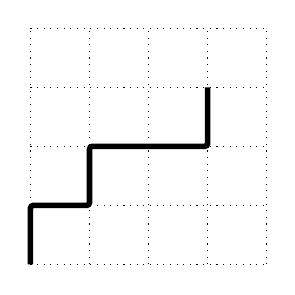
\begin{tikzpicture}[scale=.75]
  \draw[dotted] (0, 0) grid (4, 4);
  \draw[rounded corners=1, color=black, line width=2] (0, 0) -- (0, 1) -- (1, 1) -- (1, 2) -- (2, 2) -- (3, 2) -- (3, 3);
\end{tikzpicture}
\hskip .5in
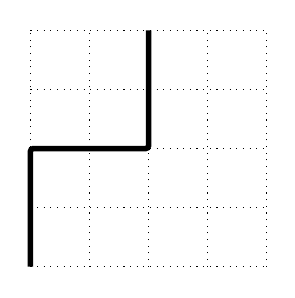
\begin{tikzpicture}[scale=.75]
  \draw[dotted] (0, 0) grid (4, 4);
  \draw[rounded corners=1, color=black, line width=2] (0, 0) -- (0, 1) -- (0, 2) -- (1, 2) -- (2, 2) -- (2, 3) -- (2, 4);
\end{tikzpicture}
\end{center}
\end{example}

The elements $G_\alpha$ are defined so that we could use them to
identify a nice basis of the ideal $I_n$.  Our first result establishes
that the $G_\alpha$ such that $\alpha$ crosses the diagonal
are in the ideal.  The slightly more difficult step is to show
that these elements also span the ideal.

\begin{prop}\label{prop:crossimpliescontains}
If $\alpha$ crosses the diagonal, then $G_\alpha \in I_n$.
\end{prop}

\begin{proof}
A sequence $\alpha \in \{ 0, 1\}^n$ is either of the form
$\alpha = 1^s0^{n-s}$ for some $s > 0$ or
$\alpha = u01^s0^{n-s-k}$ for some $s>0$ and some $u \in \{0,1\}^{k-1}$.

In the first case, $\alpha$ crosses the diagonal on the first step and
by Equation \eqref{eq:Gdef1}, $G_{1^s0^{n-s}} = F_{1^s}$
is in the ideal $I_n$.

Now the other case is established by
induction on the position of the last $1$ in $\alpha$.
We assume that
$\alpha = u01^s0^{n-s-k}$ and, by Equation \eqref{eq:Gdef2},
$G_\alpha$ is in $I_n$ if both
$G_{u1^s0^{n-k-s+1}}$ and $G_{u1^{s-1}0^{n-k-s+2}}$
are elements of $I_n$.

Assume that $u01^s0^{n-s-k}$
crosses the diagonal for the first time at position $r$.
If $r<k$, then
$u1^s0^{n-k-s+1}$ and $u1^{s-1}0^{n-k-s+2}$
both cross the diagonal also at position $r$.
Since $\alpha_k=0$, $\alpha$ does not cross the diagonal for the first
time at $r=k$, so the other possibility is that is $r>k$.
In this case $u01^{r-k}$ with $r-k \leq s$ crosses the diagonal for the first time
and therefore so does $u1^{r-k-1}$ and so do both
$u1^s0^{n-k-s+1}$ and $u1^{s-1}0^{n-k-s+2}$.
By our inductive hypothesis this implies $G_\alpha \in I_n$.

Therefore by induction, $\alpha$ crosses the diagonal implies $G_\alpha \in I_n$
for all $\alpha \in \{0,1\}^n$.
\end{proof}

We will  show that the ideal lies in the span of the $G_\alpha$ such
that $\alpha$ crosses the diagonal therefore establishing our main theorem.

\begin{theorem}\label{thm:basisofideal} 
The set $A_n:=\big\{ G_\alpha : \alpha \in \{0,1\}^n \text{ \it crosses the diagonal}\big\}$
is a $\mathbb Q$--linear basis of the ideal $I_n$.
\end{theorem}

The proof of this theorem will require a few auxiliary results and will be explained
in Section~\ref{ss:proofmainthm}.
First, we need to establish a spanning set for the quotient $EQC_n$.


\subsection{Some auxiliary results} This subsection is dedicated to the technical results we will need
to establish \ref{thm:basisofideal}.

\begin{lemma}\label{lem:spanofquotient}
The set $B_n=\big\{ \theta^\beta : \beta \in \{0,1\}^n \text{ \it stays above the diagonal}\big\}$
$\mathbb Q$--spans the quotient $R_n\big/I_n$.
\end{lemma}

\begin{proof}
Order the monomial lexicographically. Let  $\theta^\gamma$ be the smallest monomial that is not in the $\mathbb Q$--span of $B_n$
(modulo  $I_n$). We must have  that $\gamma$ crosses the  diagonal, since otherwise $\theta^\gamma\in  B_n$. Therefore, Proposition~\ref{prop:crossimpliescontains}
tells us  that $G_\gamma \in I_n$. Proposition~\ref{prop:largest} say that $G_\gamma = \theta^\gamma + \sum_{\beta<\gamma}  c_\beta \theta^\beta$. Hence, modulo $I_n$, we have
$$ \theta^\gamma \equiv \theta^\gamma - G_\gamma = - \sum_{\beta<\gamma} c_\beta \theta^\beta\,.$$
The right hand side is a linear combination of monomials strictly smaller than $\theta^\gamma$.
By the choice of $\theta^\gamma$, all such monomials are in the $\mathbb Q$--span of $B_n$.
 Therefore $\theta^\gamma$ is also in the $\mathbb Q$--span of $B_n$, a contradiction. We must conclude there are no such $\theta^\gamma$ and all monomials are in the $\mathbb Q$--span of $B_n$ modulo the ideal $I_n$.
\end{proof}

\begin{lemma}\label{lem:spanofpolynomials}
 The set ${\mathbf B}_n=\big\{ \theta^\beta F_{1^s} : \theta^\beta \in B_n,\  s\ge 0\big\}$ $\mathbb Q$--spans $R_n$.
\end{lemma}

\begin{proof} 
We show that any monomial $\theta^\gamma$ is in the span of the set ${\mathbf B}_n$.
We proceed by induction on the degree $d=m_1(\gamma)$. If $d=0$, then $\theta^\gamma = 1 = 1\cdot F_{1^0} \in {\mathbf B}_n$.
If $d>0$, we use Lemma~\ref{lem:spanofquotient} to write $\theta^\gamma$ as
$$ \theta^\gamma \equiv \sum_{\theta^\beta\in B_n}  c_\beta \theta^\beta\qquad (\text{modulo $I_n$})$$
The difference of both sides is in the ideal $I_n$ and we can write
\begin{equation}\label{eq:expansioninB}
\theta^\gamma = \sum_{\theta^\beta\in B_n}  c_\beta \theta^\beta
+ \sum_{\delta, r>0} k_{\delta,r} \theta^\delta F_{1^r}
\end{equation}
for some coefficients $k_{\delta,r}$.
This must be a homogeneous expression of degree $d$, hence $m_1(\beta) = m_1(\delta) + r = d$.
Since $r>0$, we must have that $m_1(\delta)<d$. By the induction hypothesis,
$\theta^\delta$ is in the $\mathbb Q$--span of ${\mathbf B}_n$ and we have
for some coefficients $b_{\beta,s}$ and $a_{r,s}$ from Equation~\eqref{eq:qsalg},
$$\theta^\delta F_{1^r} = \sum_{\theta^\beta\in B_n, s\ge 0} b_{\beta,s} \theta^\beta F_{1^s} F_{1^r} =  \sum_{\theta^\beta\in B_n, s\ge 0} a_{r,s} b_{\beta,s} \theta^\beta F_{1^{s+r}} \,.$$
This shows that the right hand side of~\eqref{eq:expansioninB}
is in the $\mathbb Q$--span of ${\mathbf B}_n$ which concludes the proof.
\end{proof}

\begin{lemma}\label{lem:degree}
Any monomial $\theta^\gamma$ of degree $m_1(\gamma)>\frac{n}{2}$ is in  $\mathbb Q$-span of
$A_n$ (defined in the statement of Theorem \ref{thm:basisofideal}).
\end{lemma}

\begin{proof} The proof is very similar  to Lemma~\ref{lem:spanofquotient}.
Order the monomials in $R_n$ of degree $>\frac{n}{2}$ lexicographically.
Let  $\theta^\gamma$ be the smallest such monomial that is not in $\mathbb Q$-span of $A_n$.
We have  that $\gamma$ crosses the  diagonal somewhere, since $m_1(\gamma)>\frac{n}{2}$.
Proposition~\ref{prop:largest} says that
$G_\gamma = \theta^\gamma + \sum_{\beta<\gamma}  c_\beta \theta^\beta$. Hence
$$ \theta^\gamma = G_\gamma  - \sum_{\beta<\gamma} c_\beta \theta^\beta\,.$$
The sum over $\beta$ is a linear combination of monomials that are
strictly smaller than $\theta^\gamma$. By the choice of $\theta^\gamma$,
all such monomials are in the $\mathbb Q$-span of $A_n$. 
Therefore $\theta^\gamma$ is also and this is a contradiction.
We must conclude there are no such $\theta^\gamma$ and the lemma follows.
\end{proof}


\begin{lemma}\label{lem:automorphism}
The algebra morphism $\phi\colon R_n\to R_n$ define by $\phi(\theta_i)=\theta_{n-i+1}$
is an automorphism of quasisymmetric functions. More specifically,
\begin{equation}\label{eq:autoquasi}
\phi(F_{1^s})=(-1)^{s \choose 2} F_{1^s}\,.
\end{equation}
\end{lemma}

\begin{proof} 
For any monomial $\theta_A = \theta_{a_1}\theta_{a_2}\cdots \theta_{a_s}$ such that $a_1<a_2<\cdots a_s$, we have
$$\phi(\theta_A) =  \theta_{n-a_1+1}\theta_{n-a_2+1}\cdots \theta_{n-a_s+1}
= (-1)^{s \choose 2}  \theta_{n-a_s+1}\cdots\theta_{n-a_{2}+1} \theta_{n-a_1+1}
= (-1)^{s \choose 2} \theta_{A'}$$
where $A'=\big\{ n-a_s+1< n-a_{2}+1<n-a_1+1\big\}$.
The bijection $A\leftrightarrow A'$ induces a bijection on all sets of cardinality $s$, thus
$$\phi(F_{1^s})= \sum_{|A|=s} \phi(\theta_A) =  (-1)^{s \choose 2} \sum_{|A'|=s} \theta_{A'}=(-1)^{s \choose 2} F_{1^s}\,.$$
\vskip-18pt \end{proof}

\begin{lemma}\label{lem:idealpres}
For $B_n$ given in Lemma~\ref{lem:spanofquotient}, $I_n$ is the ${\mathbb Q}$-span of the set
\begin{equation}\label{eq:autoquasi}
\big\{ \phi(\theta^\beta) F_{1^r} : \theta^\beta \in B_n,\ r>0\big\}\,.
\end{equation}
\end{lemma}

\begin{proof} Using Lemma~\ref{lem:spanofpolynomials} we have
\begin{align*}
 I_n &=  {\mathbb Q}\text{\rm -span}\big\{  \theta^\beta F_{1^s} F_{1^{r'}} :  \theta^\beta \in B_n,\  s\ge 0,\  r'>0\big\}\\
       &=  {\mathbb Q}\text{\rm -span}\big\{  \theta^\beta F_{1^{r}} :  \theta^\beta \in B_n,\  r=s+r'>0\big\}\,.
 \end{align*}
We have $\phi\big(\theta^\beta F_{1^r}\big)=\phi(\theta^\beta) \phi\big(F_{1^r}\big) = \pm \phi(\theta^\beta) F_{1^r}$, and the lemma holds.
\end{proof}

\begin{lemma}\label{lem:phiB}
For $\theta^\beta\in B_n$ as given in Lemma~\ref{lem:spanofquotient}, we have that $\phi(\theta^\beta)=\theta_{k_m} \theta_{k_{m-1}}\cdots \theta_{k_1}$
for $k_m>k_{m_1}>\cdots >k_1$ and
\begin{equation}\label{eq:phiB}
k_i  \le  n-2m+2i-1\,.
\end{equation}
\end{lemma}

\begin{proof} Let $\theta^\beta=\theta_{j_1} \theta_{j_2}\cdots \theta_{j_m}$ where $m=m_1(\beta)$ and 
$1<j_1< j_2\cdots <j_m\le n$. Recall that $\beta$ stays above the diagonal
if $\sum_{i=1}^h \beta_i\le \frac{h}{2}$.  For $h=j_\ell$, we have
 $\ell=\sum_{i=1}^{j_\ell} \beta_i \le \frac{j_\ell}{2}$.
For $\phi(\theta^\beta)=\theta_{n-j_1+1} \theta_{n-j_2+1}\cdots \theta_{n-j_m+1}=\theta_{k_m} \theta_{k_{m-1}}\cdots \theta_{k_1}$, we have
 $$  k_i = n-j_{m-i+1}+1 \le n-2(m-i+1)+1 = n-2m+2i-1.
 $$
\vskip-18pt \end{proof}


%%%%%%%%%%%%%%%%% 
\subsection{Proof of Theorem~\ref{thm:basisofideal}}\label{ss:proofmainthm}
Let ${\mathbb Q}A_n$ be the ${\mathbb Q}\text{-span}$ of the elements of $A_n$.
From Proposition~\ref{prop:crossimpliescontains} we know that
$${\mathbb Q}A_n \subseteq I_n\,.$$
Furthermore, using Proposition~\ref{prop:largest}, we know that
the elements of $A_n$ are linearly independent.
We must now show that $I_n\subseteq {\mathbb Q}A_n$. Using Lemma~\ref{lem:idealpres} it is sufficient to show that $\phi(\theta^\beta) F_{1^r}\in {\mathbb Q}A_n$ for any $ \theta^\beta \in B_n$ and
$r>0$. If $r+m_1(\beta)>\frac{n}{2}$, then Lemma~\ref{lem:degree} gives us the desired result.
We can therefore assume that $0<r\le \frac{n}{2}$  and $\theta^\beta \in B_n$
such that $m=m_1(\beta)\le \frac{n}{2}-r$.  Using Lemma~\ref{lem:phiB}, we have
\begin{equation}\label{eq:thetaF}
	\phi(\theta^\beta) F_{1^r} =  \theta_{k_m} \Big(\!\!\cdots\!  \big(\theta_{k_2} (\theta_{k_1}F_{1^r})\big)\!\cdots\!\Big)\,.
\end{equation}
The reversal of order in Equation~\eqref{eq:thetaF}, is crucial in the proof.
The idea is to start with $F_{1^r}\in {\mathbb Q}A_n$  and  show that
the succession of multiplications by $\theta_{k_i}$ in Equation~\eqref{eq:thetaF}  preserve the property of being in ${\mathbb Q}A_n$. 
The following two lemmas achieve this task and complete the proof of Theorem~\ref{thm:basisofideal}.

\begin{lemma}\label{lem:thetaG} 
 Given $\theta_k$ and $G_\gamma\in A_n$, let $u=\gamma_1\gamma_2\cdots\gamma_{k-1}$.  If 
 \begin{align*}
 	(a)_k&:\quad \gamma = u1^{s}0^{n-k-s+1}\text{ for some }s\ge 0,\\
	(b)_k&:\quad k+s+1\le n,
 \end{align*}
 then $\theta_kG_\gamma =(-1)^{m_1(u)}\big( G_{u1^{s+1}0^{n-k-s}} - G_{u01^{s+1}0^{n-k-s-1}} \big)$ where $G_{u1^{s}0^{n-k-s}},G_{u01^{s}0^{n-k-s-1}}\in A_n$. Moreover the
 position of the last $1$ in $u1^{s}0^{n-k-s}$ and $u01^{s}0^{n-k-s-1}$ is $\le k+s+1$. 
\end{lemma}

\begin{proof}
For $u1^{s}0^{n-k-s+1}=\gamma$ we
note that rearranging the terms in Equation \eqref{eq:Gdef2} and substituting $s\leftarrow s+1$ we obtain
\begin{equation}\label{eq:thetaG}
    \theta_k G_\gamma =  \theta_k G_{u1^{s}0^{n-k-s+1}} = (-1)^{m_1(u)}\big( G_{u1^{s+1}0^{n-k-s}} - G_{u01^{s+1}0^{n-k-s-1}} \big)\,.
\end{equation}
Since $k+s+1\le n$, the term on the right hand side  are well defined and 
if $u1^{s-1}0^{n-k-s+2}$ crosses the diagonal then both
$u1^{s}$ and $u01^{s}$ cross the diagonal. Therefore $G_{u1^{s}0^{n-k-s}}$ and $G_{u01^{s}0^{n-k-s-1}}$ are in $A_n$. Moreover, the position of the last $1$ in $u1^{s}0^{n-k-s}$ is $k+s<k+s+1$, and in $u01^{s}0^{n-k-s-1}$ it is $k+s+1$.
\end{proof}

\begin{lemma}\label{lem:full} 
For any $0<r\le \frac{n}{2}$  and $\theta^\beta \in B_n$ such that $m=m_1(\beta)\le \frac{n}{2}-r$, we have $\phi(\theta^\beta) F_{1^r} \in  {\mathbb Q}A_n$.
\end{lemma}

\begin{proof} We use Equation~\eqref{eq:thetaF} successively in combination with Lemma~\ref{lem:thetaG}.

\medskip
\noindent{\bf Step$_0$}:
We start with $\gamma^{(0)}=1^r0^{n-r}$ and remark that $F_{1^r}=G_{\gamma^{(0)}}\in A_n$. If $m=0$, then we are done.

\medskip
\noindent{\bf Step$_1$}: Assume $m\ge 1$.

If $k_1\le r$, then let $\gamma^{(0)}=u1^{r-k_1+1}0^{n-r}$ in Lemma~\ref{lem:thetaG}. The condition $(a)_{k_i}$ is satisfied and for $(b)_{k_i}$ we have
$k+s+1=r+2\le 2(r+m)\le 2\big(\frac{n}{2}\big)\le n$. We get $G_{1^{r+1}0^{n-r-1}}$ and $G_{1^{k_1-1}01^{r-k_1+1}0^{n-r-2}}$ in $A_n$.

If $k_1>r$, then let $\gamma^{(0)}=u0^{n-k_1+1}$ in Lemma~\ref{lem:thetaG}.  The condition $(a)_{k_i}$ is satisfied (with $s=0$) and for $(b)_{k_i}$ we have
$k_1+1\le (n-2m+2-1)+1\le (n-1)+1=n$. We get $G_{1^{r}0^{k_1-r-1}10^{n-k_1}}$ and $G_{1^{r}0^{k_1-r-1}010^{n-k_1-1}}$ in $A_n$.


At the end of Step$_1$, we have $\theta_{k_1}G_{\gamma^{(0)}}\in {\mathbb Q}A_n$. If $m=1$, then we are done. If not, all term $G_{\gamma^{(1)}}$ obtained in the product $\theta_{k_1}G_{\gamma^{(0)}}$ above,  satisfy that  for all $k>k_1$, we have
$\gamma^{(1)} = u1^{s}0^{n-k-s+1}$ for some $s\ge 0$;
and the position of the last $1$ in $\gamma^{(1)}$ is  less than or equal to $\max(r+2,k_1+1)\le n$.

We proceed by induction on $1\le j<m$ and assume that after Step$_{j}$ all terms $G_{\gamma^{(j)}}$  in the product $\theta_{k_{j}}\cdots\theta_{k_1}G_{\gamma^{(0)}}$
are in $A_n$ and satisfy
 \begin{align*}
 	(a')_{k_{j}}&:\quad \text{for all $k>k_{j}$,\ } \gamma^{(j)} = u1^{s}0^{n-k-s+1}\text{ for some }s\ge 0,\\
	(b')_{k_{j}}&:\quad \text{the position of the last $1$ in $\gamma^{(j)}$ is  less than or equal to}\\
	&\hskip .4in M_{k_j}=\max\big(r+2j,k_i+2(j-i)+1\big)_{1\le i\le j}\le n,
 \end{align*}
This is certainly the case for Step$_0$ and Step$_1$.

\medskip
\noindent{\bf Step$_{j+1}$}: Assume $m\ge j+1$. Remark that $k_{j+1}>k_j$ and using $(a')_{k_{j}}$ with $k=k_{j+1}$ we get that condition $(a)_{k_{j+1}}$ of Lemma~\ref{lem:thetaG} is satisfied and $\gamma^{(j)} = u1^{s}0^{n-k_{j+1}-s+1}$ { for some } $s\ge 0$.

If $k_{j+1}\le M_{k_j}$, then $s>0$ and $k_{j+1}+s-1$ is $M_{k_j}$. Therefore $k_{j+1}+s+1=M_{k_j}+2=\max\big(r+2j+2,k_i+2(j-i)+3\big)_{1\le i\le j}$. We have
\begin{align}
 r+2j+2&\le  2(r+m)\le 2\big({\textstyle \frac{n}{2}}\big)\le n \label{eq:rplus}\\
 k_i+2(j+1-i)+1&\le (n-2m+2i-1)+2(j+1)-2i+1 \label{eq:kplus}\\
&=n-2m+2(j+1)\le n\,. \notag
 \end{align}
 This shows that $k_{j+1}+s+1=M_{k_j}+2\le n$.
We can apply Lemma~\ref{lem:thetaG} and obtain $G_{u1^{s+1}0^{n-k_{j+1}-s}}$ and $G_{u01^{s+1}0^{n-k_{j+1}-s-1}}$ in $A_n$.

If $k_{j+1}> M_{k_j}$, then $s=0$. Using Equation~\ref{eq:kplus} with $i=j+1$ we get $k_{j+1}+s+1=k_{j+1}+1\le n$.
Again we can apply Lemma~\ref{lem:thetaG} and obtain $G_{u10^{n-k_{j+1}-s}}$ and $G_{u010^{n-k_{j+1}-s-1}}$ in $A_n$.

At the end of Step$_{j+1}$, we get that $\theta_{k_{j+1}}\theta_{k_{j}}\cdots\theta_{k_1}G_{\gamma^{(0)}}\in {\mathbb Q} A_n$. Moreover all terms $G_{\gamma^{(j+1)}}$ obtained in that product (as above) satisfy conditions $(a')_{k_{j+1}}$ and $(b')_{k_{j+1}}$  as required with
 $$M_{k_{j+1}}=\max(M_{k_j}+2,k_{j+1}+1) = \max\big(r+2(j+1),k_i+2(j+1-i)+1\big)_{1\le i\le j+1}\le n\,.$$
If $m=j+1$ we are done, if not we continue the induction.
This concludes our proof.
\end{proof}

\vskip 1in

\begin{thebibliography}{999}

\bibitem{AB} J. C. Aval, N. Bergeron,
\textit{Catalan paths and quasi-symmetric functions}.
Proc. of the Am. Math. Soc., 2003, 131(4), pp. 1053--1062.
\href{https://doi.org/10.1090/S0002-9939-02-06634-0}{10.1090/S0002-9939-02-06634-0}.

\bibitem{ABB} J. C. Aval, F. Bergeron, N. Bergeron,
\textit{Ideals of quasi-symmetric functions and super-covariant polynomials for $S_n$}.
Adv. in Math., 2004, 181 (2), pp. 353--367.
\href{https://doi.org/10.1016/S0001-8708(03)00068-9}{10.1016/S0001-8708(03)00068-9}.

\bibitem{CLO} D. Cox, J. Little, D. O'Shea,
\textit{Ideals, varieties, and algorithms: an introduction to computational
algebraic geometry and commutative algebra}.
Springer Science \& Business Media; 2013 Mar 9.

\bibitem{FLP}
Susanna Fishel, Luc Lapointe and Mar\'{\i}a Elena Pinto,
\textit{Hopf algebra structure of symmetric and quasisymmetric
              functions in superspace}.
 {J. Combin. Theory Ser. A}, 2019, 166, pp.  {144--170}.
\href{https://doi-org/10.1016/j.jcta.2019.02.016}{10.1016/j.jcta.2019.02.016}.

\bibitem{H} F. Hivert, 
\textit{Hecke algebras, difference operators, and quasi-symmetric
              functions}.
Adv. in Math., 2000, 155 (2), pp. 181--238.
\href{https://doi-org/10.1006/aima.1999.1901}{10.1006/aima.1999.1901}.

\bibitem{L} S. X. Li,
\textit{Ideals and quotients of diagonally quasi-symmetric functions}.
Elec. J. Comb., Vol 24, Issue \#3, P3.3.
\href{https://doi.org/10.37236/6658}{10.37236/6658}.
\end{thebibliography}

\end{document}


